\section{Installation}
\label{sec:installation}

\subsection{Windows}

In order to successfully follow the examples in this manual and use
\emph{DSLTrans} you have to follow these steps carefully:

\subsubsection{Step 1}
Make sure you have java 1.6 or Java 1.7 installed. DSLTrans is not yet compatible with Java 1.8.

\subsubsection{Step 2}

Download and extract Eclipse Modeling Tools, Luna Service Release 1.

\subsubsection{Step 3}
Set the environment variables shown in the Figure~\ref{fig:path_user} below.

\begin{figure}[H]
\begin{center}
  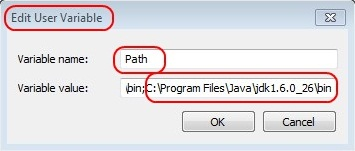
\includegraphics[scale=0.9]{imgs/path_user.jpg}
  \caption{Path to add to the \emph{user} \emph{Path} variable.}
  \label{fig:path_user}
\end{center}
\end{figure}

Note that in figure \ref{fig:path_user} you have to replace \verb=C:\Program Files\Java\jdk1.6.0_26\bin=
by your system's Java bin directory. Also, beware that the environment variable you have to edit is the \emph{user} Path variable.

\subsubsection{Step 4}

Now you have to copy the \verb=jpl.jar= file, in the 
\verb=C:\Program Files\pl\lib= 
directory, and paste it in Java's lib directory: 
\verb=C:\Program Files\Java\jdk1.6.0_26\lib=.

\begin{figure}[h]
\begin{center}
  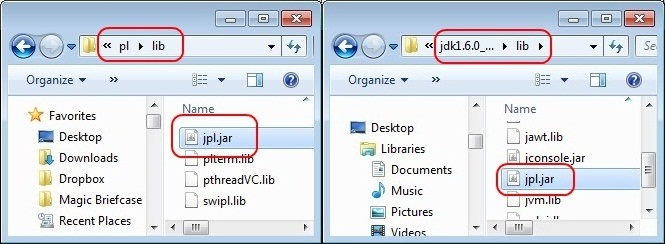
\includegraphics[width=0.8\textwidth]{imgs/jpl_cpy.jpg}
  \caption{Prolog's jpl.jar copied to Java's lib directory.}
  \label{fig:jpl_cpy}
\end{center}
\end{figure}

\subsubsection{Step 5}

Finally, you need to install the DSLTrans editor and transformer features from the DSLTrans update site.
For this, either use the update side:\\
{\scriptsize
\verb=https://dl.dropboxusercontent.com/u/9650993/UpdateSiteDSLTrans/site.xml=
}\\
, or download and extract the DSLTransUpdateSite from the \emph{DSLTrans-Release} folder in our repository and install the features to eclipse using that update site:\\
\url{https://github.com/githubbrunob/DSLTransGIT}


\subsubsection{Step 6}

Afterward, restart the pc.

\clearpage


\begin{comment}	

Download & Install Prolog

Download & Install Plugins

Handle java library path

Path do admin com C:\Program Files\pl\bin

Copy jpl.jar to lib java folder

\end{comment}



